\documentclass[11pt]{article}
\usepackage[utf8]{inputenc}
\usepackage[T1]{fontenc}
\usepackage{amsmath}
\usepackage{amssymb} % Needed for \eth
\usepackage{graphicx}
\usepackage{geometry}
\usepackage{tikz}
\usepackage{pgfplots} % For plots
\usepackage{ulem}     % For underline, using normalem to avoid messing with \emph

\geometry{a4paper, margin=1in}
\usetikzlibrary{positioning, arrows.meta, shapes.geometric} % For TikZ diagrams
\pgfplotsset{compat=1.18} % Use a recent PGFPlots version

% Custom commands (optional)
\newcommand{\avg}[1]{\overline{#1}}
\newcommand{\prob}[1]{P(#1)}
\newcommand{\ProbDens}[1]{\mathcal{P}(#1)} % Using script P for density
\newcommand{\vect}[1]{\vec{#1}}
\newcommand{\dd}[1]{\mathrm{d}#1} % Differential d
\newcommand{\pderiv}[2]{\frac{\partial #1}{\partial #2}}
\newcommand{\deriv}[2]{\frac{\mathrm{d} #1}{\mathrm{d} #2}}
\newcommand{\muState}{\mu\text{-state}} % Microstate
\newcommand{\OmegaE}{\Omega(E)}
\newcommand{\omegaE}{\omega(E)}
\newcommand{\PhiE}{\Phi(E)}
\newcommand{\deltaE}{\delta E}
\newcommand{\ethbar}{\text{\it{đ}}} % \eth symbol for inexact differential
\newcommand{\kb}{k_B} % Boltzmann constant
\newcommand{\Na}{N_A} % Avogadro constant
\newcommand{\gasR}{R} % Gas constant

\title{Physics 415 - Lecture 11: Ideal Gas Applications}
\date{February 14, 2025}
\author{} % Author not specified

\begin{document}

\maketitle
\thispagestyle{empty}

\section*{Summary}

\begin{itemize}
    \item Equilibrium macro system: $dE = T dS - p dV$, with $E=E(S,V)$.
    \item First Law of Thermo: $dE = \ethbar Q - \ethbar W$.
    \item For quasi-static process: $\ethbar W = p dV$ and $\ethbar Q = T dS$.
    \item Heat Capacity: $\ethbar Q|_x = C_x dT$. $C_x$ = heat capacity at constant $x$.
    \item $C_x = T \left( \pderiv{S}{T} \right)_x$. Allows finding entropy change at fixed $x$:
    \[ \Delta S = S(x, T_2) - S(x, T_1) = \int_{T_1}^{T_2} dT \frac{C_x(T)}{T} \]
    (Measuring $C_x(T)$ determines changes in $S$).
\end{itemize}

\section*{Ideal Gas}

Definition: A gas in which interactions between particles are so weak they can be neglected.
\begin{itemize}
    \item Usually achieved in the limit of dilute gases, where particles are almost always far apart, so interaction forces are small.
\end{itemize}
Ideal gas equation of state:
\[ pV = N T \]
(where $T$ is in energy units).
Alternatively, using $T$ in Kelvin (degrees):
\[ pV = N \kb T \]
We can also write this in terms of moles: $N = \nu \Na$, where $\nu=$ \# moles and $\Na = 6.02 \times 10^{23}$ mol$^{-1}$ (Avogadro's number).
\[ pV = \nu (\Na \kb) T \]
Let $\gasR = \Na \kb \approx 8.314$ J/(mol·K) be the ideal gas constant.
\[ pV = \nu \gasR T \]
We previously derived the equation of state $pV=NT$ from the microscopic calculation $\Omega(E,V) \propto V^N E^{3N/2}$ for a classical monatomic ideal gas.

\subsection*{Energy of Ideal Gas}

Earlier, we showed from microscopic considerations that $E = \frac{3}{2} N T$ (monatomic). As a first application of macroscopic thermodynamics, let's re-derive the result that $E$ depends only on $T$, i.e., $E=E(T)$, independent of $V$, using only the equation of state $pV=NT$ and general thermodynamic relations.

Take $(T, V)$ as independent variables, so $E=E(T,V)$ in general.
\[ dE = \left( \pderiv{E}{T} \right)_V dT + \left( \pderiv{E}{V} \right)_T dV \]
Also, from the fundamental relation $dE = T dS - p dV$, we can write $dS = \frac{1}{T} dE + \frac{p}{T} dV$.
Considering $S=S(T,V)$:
\[ dS = \left( \pderiv{S}{T} \right)_V dT + \left( \pderiv{S}{V} \right)_T dV \]
Substitute $dE$ into the expression for $dS$:
\[ dS = \frac{1}{T} \left[ \left( \pderiv{E}{T} \right)_V dT + \left( \pderiv{E}{V} \right)_T dV \right] + \frac{p}{T} dV \]
\[ dS = \frac{1}{T} \left( \pderiv{E}{T} \right)_V dT + \left[ \frac{1}{T} \left( \pderiv{E}{V} \right)_T + \frac{p}{T} \right] dV \]
Comparing the coefficients of $dT$ and $dV$ with the expression for $dS$ in terms of $T, V$:
\[ \left( \pderiv{S}{T} \right)_V = \frac{1}{T} \left( \pderiv{E}{T} \right)_V \]
\[ \left( \pderiv{S}{V} \right)_T = \frac{1}{T} \left( \pderiv{E}{V} \right)_T + \frac{p}{T} \]
Now use the equality of mixed second partial derivatives: $\pderiv[2]{S}{V \partial T} = \pderiv[2]{S}{T \partial V}$.
\[ \pderiv{}{V} \left[ \left( \pderiv{S}{T} \right)_V \right]_T = \pderiv{}{T} \left[ \left( \pderiv{S}{V} \right)_T \right]_V \]
\[ \pderiv{}{V} \left[ \frac{1}{T} \left( \pderiv{E}{T} \right)_V \right]_T = \pderiv{}{T} \left[ \frac{1}{T} \left( \pderiv{E}{V} \right)_T + \frac{p}{T} \right]_V \]
The derivative $\partial/\partial V$ acts on $(\partial E/\partial T)_V$. The derivative $\partial/\partial T$ acts on $1/T$, $(\partial E/\partial V)_T$, and $p/T$.
\[ \frac{1}{T} \pderiv[2]{E}{V \partial T} = -\frac{1}{T^2} \left( \pderiv{E}{V} \right)_T + \frac{1}{T} \pderiv[2]{E}{T \partial V} + \pderiv{}{T} \left( \frac{p}{T} \right)_V \]
Since mixed partials of $E$ are equal, the terms with $\partial^2 E$ cancel:
\[ 0 = -\frac{1}{T^2} \left( \pderiv{E}{V} \right)_T + \pderiv{}{T} \left( \frac{p}{T} \right)_V \]
\[ \implies \left( \pderiv{E}{V} \right)_T = T^2 \pderiv{}{T} \left( \frac{p}{T} \right)_V \]
This is a general thermodynamic result.
Now, apply it to an ideal gas. From $pV=NT$, we have $p/T = N/V$.
\[ \pderiv{}{T} \left( \frac{p}{T} \right)_V = \pderiv{}{T} \left( \frac{N}{V} \right)_V = 0 \]
(since $N/V$ is independent of $T$ at constant $V$).
\[ \implies \left( \pderiv{E}{V} \right)_T = 0 \]
This proves from macroscopic thermodynamics (using the ideal gas law) that the internal energy $E$ of an ideal gas is independent of volume $V$; it depends only on temperature $T$.
\[ E = E(T) \quad (\text{Ideal Gas}) \]

\subsection*{Heat Capacity / Specific Heat of Ideal Gas}

Define molar specific heat $c_x = C_x / \nu$ (heat capacity per mole). $C_x$ is extensive, $c_x$ is intensive.

\textbf{Constant Volume:}
$\ethbar Q|_V = C_V dT = \nu c_v dT$.
From First Law, $\ethbar Q|_V = dE|_V + \ethbar W|_V$. Since $dV=0$, $\ethbar W|_V = 0$.
$\ethbar Q|_V = dE|_V$. Since $E=E(T,V)$ generally, $dE = (\partial E/\partial T)_V dT + (\partial E/\partial V)_T dV$.
$dE|_V = (\partial E/\partial T)_V dT$.
$\implies \nu c_v dT = (\partial E/\partial T)_V dT$.
\[ c_v = \frac{1}{\nu} \left( \pderiv{E}{T} \right)_V \quad (\text{General result}) \]
Note: Since stability requires $T$ to increase with $E$ (usually), $\partial E / \partial T > 0$, so $c_v > 0$.

For an ideal gas, $E=E(T)$ only. $\implies (\partial E/\partial T)_V = dE/dT$.
\[ dE = \nu c_v dT \quad (\text{Ideal Gas}) \]
This means for an ideal gas, the change in energy depends only on the temperature change, regardless of the process.

\textbf{Constant Pressure:}
$\ethbar Q|_p = C_p dT = \nu c_p dT$.
First Law: $\ethbar Q|_p = dE|_p + \ethbar W|_p = dE|_p + p dV|_p$.
For an ideal gas, $dE = \nu c_v dT$.
From $pV = \nu \gasR T$, at constant $p$: $p dV|_p = \nu \gasR dT|_p$.
Substitute these into the First Law expression for $\ethbar Q|_p$:
\[ \nu c_p dT = (\nu c_v dT) + (\nu \gasR dT) \]
\[ \implies c_p = c_v + \gasR \quad (\text{Ideal Gas}) \]
Note: $C_p = C_V + \nu \gasR$. Since $R>0$, we have $c_p > c_v$. This is because at constant pressure, some added heat goes into doing expansion work ($pdV$), whereas at constant volume all added heat goes into increasing internal energy $E$.

\subsection*{Microscopic View (Monatomic Ideal Gas)}

This is as much as we can say from macro theory alone (plus ideal gas law). We also know $c_v = c_v(T)$ since $E=E(T)$. To say more, we need microscopic input.

Recall: For classical monatomic ideal gas, $E = \frac{3}{2} N T = \frac{3}{2} \nu \gasR T$. (Using $T$ in Kelvin now for $R$).
Using $c_v = \frac{1}{\nu} (\partial E / \partial T)_V = \frac{1}{\nu} (dE/dT)$:
\[ c_v = \frac{1}{\nu} \deriv{}{T} \left( \frac{3}{2} \nu \gasR T \right) = \frac{3}{2} \gasR \]
This is a constant, independent of $T$.
Then $c_p = c_v + \gasR = \frac{3}{2} \gasR + \gasR = \frac{5}{2} \gasR$.
The ratio of specific heats (adiabatic index) is:
\[ \gamma \equiv \frac{c_p}{c_v} = \frac{5/2 \gasR}{3/2 \gasR} = \frac{5}{3} \]
($\gamma$ can be measured from the speed of sound in the gas).

For polyatomic gases, $c_v$ is generally larger (due to rotational, vibrational DOF) and can depend on $T$ as different DOFs become active. This dependence involves QM effects.

\begin{center}
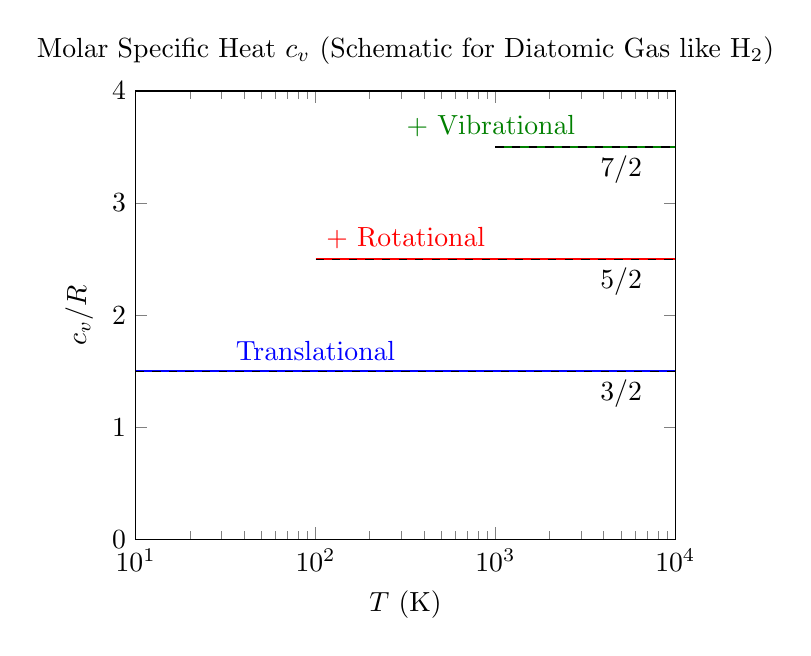
\begin{tikzpicture}
\begin{axis}[
    xlabel={$T$ (K)},
    ylabel={$c_v / \gasR$},
    xmode=log, % Log scale for Temperature
    xmin=10, xmax=10000,
    ymin=0, ymax=4,
    legend pos=north west,
    title={Molar Specific Heat $c_v$ (Schematic for Diatomic Gas like H$_2$)}
]
% Translational part (3/2 R)
\addplot [domain=10:10000, thick, blue, const plot] {1.5} node [pos=0.5, anchor=south east] {Translational};
% Add rotational part (+2/2 R = R) above ~100K
\addplot [domain=100:10000, thick, red, const plot] {1.5+1.0} node [pos=0.5, anchor=south east] {+ Rotational};
% Add vibrational part (+2/2 R = R) above ~1000K
\addplot [domain=1000:10000, thick, green!50!black, const plot] {1.5+1.0+1.0} node [pos=0.5, anchor=south east] {+ Vibrational};

% Indicate levels
\draw [dashed] (axis cs:10, 1.5) -- (axis cs:10000, 1.5); \node at (axis cs:5000, 1.3) {$3/2$};
\draw [dashed] (axis cs:100, 2.5) -- (axis cs:10000, 2.5); \node at (axis cs:5000, 2.3) {$5/2$};
\draw [dashed] (axis cs:1000, 3.5) -- (axis cs:10000, 3.5); \node at (axis cs:5000, 3.3) {$7/2$};
\end{axis}
\end{tikzpicture}
\end{center}
However, treating $c_v$ (and hence $\gamma$) as constant is often a good approximation over broad ranges of $T$.

\section*{Processes in Ideal Gas}

Investigate ideal gas subject to various processes.

\subsection*{Isothermal Expansion}
Quasi-static process at constant $T$.
From $pV = \nu \gasR T = \text{const}$, we have $p V = \text{constant}$, or $p \propto 1/V$.

\subsection*{Adiabatic Expansion}
Quasi-static process with no heat transfer ($\ethbar Q = 0$).
Gas will change energy ($\implies$ change $T$) by doing work.
What is the relationship between $p$ and $V$ for such a process?

First Law: $\ethbar Q = dE + \ethbar W \implies 0 = dE + p dV$.
For ideal gas, $dE = \nu c_v dT$.
So, $\nu c_v dT + p dV = 0$.

We need to relate $dT$ to $p, V$. Use equation of state $pV = \nu \gasR T$.
Differentiate: $p dV + V dp = \nu \gasR dT$.
Solve for $dT$: $dT = \frac{p dV + V dp}{\nu \gasR}$.
Substitute into the First Law equation:
\[ \nu c_v \left( \frac{p dV + V dp}{\nu \gasR} \right) + p dV = 0 \]
\[ \frac{c_v}{\gasR} (p dV + V dp) + p dV = 0 \]
\[ \left( \frac{c_v}{\gasR} + 1 \right) p dV + \frac{c_v}{\gasR} V dp = 0 \]
Use $c_p = c_v + \gasR \implies c_p/\gasR = c_v/\gasR + 1$.
\[ \left( \frac{c_p}{\gasR} \right) p dV + \left( \frac{c_v}{\gasR} \right) V dp = 0 \]
Multiply by $\gasR$:
\[ c_p p dV + c_v V dp = 0 \]
Divide by $c_v p V$ (assuming $p, V, c_v \neq 0$):
\[ \frac{c_p}{c_v} \frac{dV}{V} + \frac{dp}{p} = 0 \]
Let $\gamma = c_p / c_v$.
\[ \gamma \frac{dV}{V} + \frac{dp}{p} = 0 \qquad (*) \]
Assuming $\gamma$ is constant (which is true for monatomic ideal gas, and approx true for others over ranges of T), we can integrate $(*)$:
\[ \gamma \int \frac{dV}{V} + \int \frac{dp}{p} = \text{constant} \]
\[ \gamma \ln V + \ln p = \text{constant} \]
\[ \ln(p V^\gamma) = \text{constant} \]
\[ \implies p V^\gamma = \text{constant} \quad (\text{Adiabatic process for Ideal Gas}) \]
This relates $p$ and $V$ during a quasi-static adiabatic process.
Using $pV=NT$, we can also write $T V^{\gamma-1} = \text{constant}$.

In an adiabatic process, $p \propto V^{-\gamma}$. Since $\gamma = c_p/c_v > 1$, pressure varies more rapidly with $V$ than for an isothermal process where $p \propto V^{-1}$.

\end{document}